\documentclass[12pt, a4paper]{article}
\usepackage[utf8]{inputenc}
\usepackage[T1]{fontenc}
\usepackage[slovene]{babel}
\usepackage{amsmath}
\usepackage{eurosym}
\usepackage{hyperref}
\usepackage{graphicx}
\usepackage[top=2.5cm, bottom=2.5cm, left=3cm, right=2.5cm]{geometry}
\usepackage{indentfirst}
\usepackage{tikz}
\setlength{\parindent}{0.5cm}


\begin{document}

\begin{titlepage}
\begin{center}

\large
Univerza v Ljubljani\\
\normalsize
Fakulteta za matematiko in fiziko\\

\vspace{3 cm} 

\large
Žan Jernejčič in Ines Šilc\\

\vspace{0.5cm}
\LARGE
\textbf{Reševanje problema trgovskega potnika s k-optimalnim in
Lin-Kernighanovim algoritmom}

\vfill

\large Ljubljana, 2020

\end{center}
\end{titlepage}

\newpage

\section[Definiranje problema]{Definiranje problema}

V projektni nalogi bova reševala Problem trgovskega potnika s pomočjo k-optimalnega in Lin-Kernighanovega algoritma.\\

Problem trgovskega potnika oziroma Travelling salesman problem (krajše TSP) je problem, kjer imamo podanih $n$ mest in razdalje med vsemi (za vsak par mest imamo torej podano, koliko sta si oddaljeni). Zanima nas, ali lahko obiščemo vsako mesto in se na koncu vrnemo v prvotno mesto. Če označimo $d_{i, j}$ kot razdaljo mad $i$-tim in $j$-tim mestom, iščemo torej:

$$
\min_{\pi \in S_n} \sum\limits_{i=1}^{n-1} d_{\pi (i), \pi (i+1)} + d_{\pi (n), \pi (1)}
$$
 kjer je $S_n$ množica vseh permutacij danih $n$ mest. \\
 
Naivna rešitev je očitna, pogledamo $(n-1)!$ kombinacij, torej iz vsakega mesta v vsako drugo mesto, si zapišemo vse kombinacije in kakšno razdaljo smo prepotovali, ter izberemo tisto možnost, kjer je bila razdalja najkrajša.\\ 

Pred začetkom se lahko vprašamo kakšen mora biti graf, da lahko na njem izvajamo sledeča algoritma. Graf \textbf{ne sme} imeti \textbf{negativnih ciklov}, saj je najcenejši cikel potem očiten, in ustvarimo neskončno zanko, saj bo imela najboljša rešitev ceno -$\infty$. Ker imamo opravka s cikli, lahko cikel začnemo v kateremkoli vozlišču, zato lahko vedno gledamo možne poti od začetka.\\

Za projekt sva uporabila programski jezik \texttt{python}. Uporabljala sva naslednje pakete:

\begin{itemize}

\item \texttt{networkx}: za definiranje in generiranje grafov

\item \texttt{random}: za generiranje naključnih števil in seznamov

\item \texttt{matplotlib}: za izrisovanje grafov

\item \texttt{timeit}: za mertive časovne zahtevnosti

\item \texttt{itertools}: za generiranje prvotne permutacije

\end{itemize}

Za preverjanje veljavnosti poti v grafu za problem potujočega trgovca, morava vedeti:

\begin{itemize}

\item Vsaka pot trgovca bo morala imeti vsa vozlišča primarnega grafa
\item Vsaka pot trgovca bo morala imeti točno toliko povezav kot vozlišč
\item Dolžina poti bo morala biti enaka številu vozlišč -1

\end{itemize}

\newpage
\section[k-optimalni algoritmi]{k-optimalni algoritmi}

K-optimalni algoritem, je lokalni algoritem, kjer iščemo rešitev Problema trgovskega potnika in sorodnih problemov. Algoritem deluje tako, da zmanjša dolžino trenutnega potovanja, dokler ne dosežemo poti, katere dolžine ne moremo izboljšati.\\

Poznamo več različic k-opt algoritma. V tej projektni nalogi se bova osredotočila na dve glavni različici k-opt algoritma, to sta 2-Opt in 3-Opt algoritem. 2-Opt algoritem deluje tako, da odstrani dve vozlišči grafa (dve mesti), tako razdeli pot na dva dela, poišče najboljšo rešitev podproblema, in nato poveže nazaj mesti na najboljši možen način. 3-Opt algoritem odstrani tri povezave ali vozlišča, tako dobimo 3 podomrežja mest. V naslednjem koraku analiziramo najboljšo pot med temi tremi podomrežji. To ponavljamo za druge tri povezave, dokler nismo poskusili vseh možnih poti v danem omrežju.

\subsection[2-opt algoritem]{2-opt algoritem}

Za začetek 2-opt postopka potrebujemo poln graf z utežmi na vsaki povezavi in danim začetnim ciklom po tem grafu. Postopoma odstranjujemo po dve vozlišči in ju povežemo drugače, nato preverimo, ali je novonastali cikel cenejši. Če je novi cikel cenejši, potem ga vzamemo za boljšo rešitev. Ta postopek nadaljujemo, dokler ne pridemo do konca poti in se moramo vrniti na začetek. \\

Za algoritem potrebujemo še dodatno funkcijo, ki nam izračuna ceno poti, ta prejme vhodne podatke graf in pot in sešteje uteži poti v grafu. Dejanski postopek 2-opt algoritma izgleda takole:
\begin{verbatim}
def dva_opt(graf, pot):

    najboljsa_pot = pot
    
    cena = cena_poti(graf, pot)

    izboljsanje = True
    while izboljsanje:
        izboljsanje = False
        for i in range(1,len(pot) - 2):

            for j in range(i + 1, len(pot)):
 
                if j - i == 1: continue
                nova_pot = pot[:]
                nova_pot[i:j] = pot[j - 1:i - 1:-1]
                nova_cena = cena_poti(graf, nova_pot)

                if nova_cena < cena:
                    najboljsa_pot = nova_pot[:]
                    cena = nova_cena
                    izboljsanje = True
        pot = najboljsa_pot

    return (pot, cena)

\end{verbatim}

Algoritem gre postopoma po poti in zamenja zaporedje vozlišč, če je le tako bolj optimalno. Dva koraka 2-opt algoritma bi izgledala takole:\\

\begin{minipage}{0.3\textwidth}
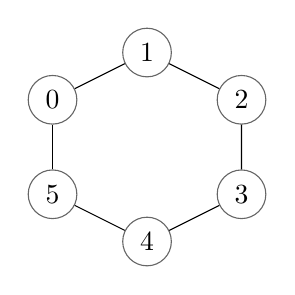
\begin{tikzpicture}
  [scale=.3,auto=left,every node/.style={circle, draw = black!60}]
  \node (n0) at (1,8) {0};
  \node (n1) at (5,10)  {1};
  \node (n2) at (9,8)  {2};
  \node (n5) at (1,4) {5};
  \node (n4) at (5,2)  {4};
  \node (n3) at (9,4)  {3};

  \foreach \from/\to in {n0/n1,n1/n2,n2/n3,n3/n4,n4/n5,n5/n0}
    \draw (\from) -- (\to);
\end{tikzpicture}
\end{minipage}
\hspace{1cm}
\begin{minipage}{0.3\textwidth}
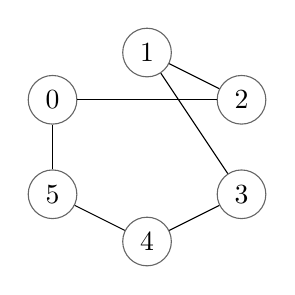
\begin{tikzpicture}
  [scale=.3,auto=left,every node/.style={circle, draw = black!60}]
  \node (n0) at (1,8) {0};
  \node (n1) at (5,10)  {1};
  \node (n2) at (9,8)  {2};
  \node (n5) at (1,4) {5};
  \node (n4) at (5,2)  {4};
  \node (n3) at (9,4)  {3};

  \foreach \from/\to in {n0/n2,n1/n2,n1/n3,n3/n4,n4/n5,n5/n0}
    \draw (\from) -- (\to);
\end{tikzpicture}
\end{minipage}
\hspace{1cm}
\begin{minipage}{0.3\textwidth}

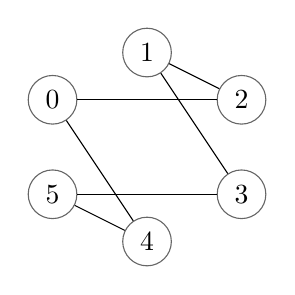
\begin{tikzpicture}
  [scale=.3,auto=left,every node/.style={circle, draw = black!60}]
  \node (n0) at (1,8) {0};
  \node (n1) at (5,10)  {1};
  \node (n2) at (9,8)  {2};
  \node (n5) at (1,4) {5};
  \node (n4) at (5,2)  {4};
  \node (n3) at (9,4)  {3};

  \foreach \from/\to in {n0/n2,n1/n2,n1/n3,n3/n5,n4/n5,n4/n0}
    \draw (\from) -- (\to);
\end{tikzpicture}
\end{minipage}\\\vspace{0.5cm}

Za primer delovanja si oglejmo preprosto matriko, ki predstavlja graf. Na $(i, j)$-tem mestu matrike je cena med mestoma $i$ in $j$. Dana je matrika (\ref{matrika}) in njen graf je narisan na sliki \ref{primeri/primer1.png}
\begin{equation}
\label{matrika}
\begin{bmatrix} 
0&2&3&4&1000\\
2&0&8&9&10\\
3&8&0&14&15\\
4&9&14&0&20\\
1000&10&15&20&0\\
\end{bmatrix}
\end{equation}

Rešitev, ki nam jo poda 2-opt algoritem je na sliki \ref{resitev_2_opt}:

\begin{figure}[!h]
    
    \begin{minipage}{0.5\textwidth}
    \includegraphics[width=7 cm]{primeri/primer1.png}
    \caption{Primer grafa}
    \label{primeri/primer1.png}
  \end{minipage}
 \hspace{1cm}
  \begin{minipage}{0.5\textwidth}
    \includegraphics[width=7 cm]{primeri/primer1_2opt.png}
    \caption{Rešitev primera z 2-opt}
    \label{resitev_2_opt}
  \end{minipage}
    
\end{figure}

Še en primer:

\begin{figure}[!h]
    
    \begin{minipage}{0.5\textwidth}
    \includegraphics[width=7 cm]{primeri/primer2.png}
    \caption{Primer grafa}
    \label{primer_2_opt_2}
  \end{minipage}
 \hspace{1cm}
  \begin{minipage}{0.5\textwidth}
    \includegraphics[width=7 cm]{primeri/primer2_2opt.png}
    \caption{Rešitev primera z 2-opt}
    \label{resitev_2_opt_2}
  \end{minipage}
    
\end{figure}


\newpage
\subsection[3-opt algoritem]{3-opt algoritem}

\begin{minipage}{0.3\textwidth}
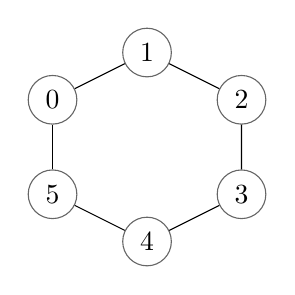
\begin{tikzpicture}
  [scale=.3,auto=left,every node/.style={circle, draw = black!60}]
  \node (n0) at (1,8) {0};
  \node (n1) at (5,10)  {1};
  \node (n2) at (9,8)  {2};
  \node (n5) at (1,4) {5};
  \node (n4) at (5,2)  {4};
  \node (n3) at (9,4)  {3};

  \foreach \from/\to in {n0/n1,n1/n2,n2/n3,n3/n4,n4/n5,n5/n0}
    \draw (\from) -- (\to);
\end{tikzpicture}
\end{minipage}
\hspace{1cm}
\begin{minipage}{0.3\textwidth}
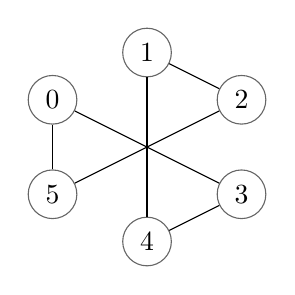
\begin{tikzpicture}
  [scale=.3,auto=left,every node/.style={circle, draw = black!60}]
  \node (n0) at (1,8) {0};
  \node (n1) at (5,10)  {1};
  \node (n2) at (9,8)  {2};
  \node (n5) at (1,4) {5};
  \node (n4) at (5,2)  {4};
  \node (n3) at (9,4)  {3};

  \foreach \from/\to in {n5/n2,n1/n2,n4/n3,n3/n0,n4/n1,n5/n0}
    \draw (\from) -- (\to);
\end{tikzpicture}
\end{minipage}

\begin{figure}[!h]
    
    \begin{minipage}{0.5\textwidth}
    \includegraphics[width=8 cm]{primeri/primer1.png}
    \caption{Primer grafa}
    \label{primer_3_opt}
  \end{minipage}
 \hspace{1cm}
  \begin{minipage}{0.5\textwidth}
    \includegraphics[width=8 cm]{primeri/primer1_3opt.png}
    \caption{Rešitev primera s 3-opt}
    \label{resitev_3_opt}
  \end{minipage}
    
\end{figure}

\begin{figure}[!h]
    
    \begin{minipage}{0.5\textwidth}
    \includegraphics[width=8 cm]{primeri/primer2.png}
    \caption{Primer grafa}
    \label{primer_3_opt}
  \end{minipage}
 \hspace{1cm}
  \begin{minipage}{0.5\textwidth}
    \includegraphics[width=8 cm]{primeri/primer2_3opt.png}
    \caption{Rešitev primera s 3-opt}
    \label{resitev_3_opt}
  \end{minipage}
    
\end{figure}




\newpage
\section[Lin-Kernighanov algoritem]{Lin-Kernighanov algoritem}
K-Opt algoritmi so vezani na fiksen k. Lin-Kernighanov algoritem pa na vsakem koraku preveri katero vrednost k se nam splača uporabiti. Začnemo s $k=2$ in naslednja vrednost je za 1 večja. Vrednost k-ja se povečuje doker ne najde zamenjave, ki izboljšata obhod, v tem primeru ponastavi  k na 2. Če take zamenjave ne najdemo potem k povečamo za 1. Če take zamenjave ne najdemo in preizkusimo vse dovoljene zamenjave, potem je dobljena rešitev lokalni ali pa celo globalni minimum.  Običajno Lin-Kernighanov algoritem ne vzame k-ja večjega od 3.\\

Primer grafa s 5 in 10 vozlišči in končne rešitve.

\begin{figure}[!h]
    
    \begin{minipage}{0.5\textwidth}
    \includegraphics[width=7 cm]{primeri/primer1.png}
    \caption{Primer grafa s 5 vozlišči}
    \label{primer_LK}
  \end{minipage}
 \hspace{1cm}
  \begin{minipage}{0.5\textwidth}
    \includegraphics[width=7 cm]{primeri/primer1_lk.png}
    \caption{Rešitev primera z LK algoritmom}
    \label{resitev_LK}
  \end{minipage}
    
\end{figure}


\begin{figure}[!h]
    
    \begin{minipage}{0.5\textwidth}
    \includegraphics[width=7 cm]{primeri/primer2.png}
    \caption{Primer grafa z 10 vozlišči}
    \label{primer_LK}
  \end{minipage}
 \hspace{1cm}
  \begin{minipage}{0.5\textwidth}
    \includegraphics[width=7 cm]{primeri/primer2_lk.png}
    \caption{Rešitev primera z LK algoritmom}
    \label{resitev_LK}
  \end{minipage}
    
\end{figure}

\newpage

\section[Časovna zahtevnost in red napake]{Časovna zahtevnost in red napake}
Pri 2-Opt algoritmu se red napake giblje med $O(\frac{\log n}{\log (\log n)} )$ in $O(\log n)$, pri 3-Opt algoritmu in Lin-Kernighanovemu algoritmu pa je enak $O(\sqrt[3]{n})$. 
\\
V teoriji je časovna zahtevnost za k-Opt algoritem enaka $O(n^{k})$, kjer je n število vozlišč v grafu. Časovna zahtevnost za Lin-Kernighanov algoritem pa je nekoliko manj kot $O(n^{3})$
V projektni nalogi sva še praktično analizirala časovno zahtevnost vsakega od treh algoritmov. To sva naredila tako, da sva merila, koliko časa vsak algoritem porabi za poln graf v odvisnosti od n. Izračunala sva čase za n = 5, 10, 100... in dobila naslednje rezultate\footnote{Pri merjenju časovne zahtevnosti je pomembno, meriva samo časovno zahtevnost algoritma in ne ostalih stvari, kot so preurejanje in izrisovanje grafa.}:


\begin{table}[!h]
\begin{tabular}{|c|c|c|c|c|c|c|c|}
\hline
n&cena začetne&2-opt&cena 2-opt&3-opt&cena 3-opt&LK&cena LK\\\hline
5&49&0,000675&41&0,000276&41&0,000154&41\\\hline
10&4903&0.004748&1595&0,000600&1484&0,000611&1484\\\hline
20&9047&0,03257&1388&0,00801&1555&0,01151&1517\\\hline
30&11825&0,10143&2255&0,01806&1907&0,04639&1729\\\hline
50&23556&0,69378&2833&0,18529&2496&0,30218&2319\\\hline
100&46984&11,3602&46984&1,97813&2446&2,31723&2235\\\hline
200&98344&194,093&4673&22,9016&3007&13,7700&2832\\\hline
300&156543&1127,92&5365&162,040&2986&94,0348&2630\\\hline
500&244733&7912.40&6689&402.52&3328&496.36&2900\\\hline
1000&483979&&&&&&\\\hline
\end{tabular}
\end{table}


\newpage
\section[Viri]{Viri}

\begin{enumerate}

\item A. Hagberg, D. Schult, P. Swart:\emph{NetworkX Refrence, Release 2.4}, [ogled 2.~1.~2020], dostopno na \url{https://networkx.github.io/documentation/stable/_downloads/networkx_reference.pdf}

\item \emph{Optimization with 2-OPT - Part 1}, [ogled 3.~1.~2020], dostopno na \url{http://pedrohfsd.com/2017/08/09/2opt-part1.html}

\item \emph{2-opt}, [ogled 3.~1.~2020], dostopno na \url{https://en.wikipedia.org/wiki/2-opt}

\item \emph{3-opt}, [ogled 4.~1.~2020], dostopno na \url{https://en.wikipedia.org/wiki/3-opt}

\item \emph{3-opt: basic algorithm}, [ogled 4.~1.~2020], dostopno na \url{https://tsp-basics.blogspot.com/2017/03/3-opt-iterative-basic-algorithm.html}
\end{enumerate}

\end{document}